%%%%%%%%%%%%%%%%%%%%%%%%%%%%%%%%%%%%%%%%%%%%%%%%%
%%         Projet Dome geodesique              %%
%%            Convention tri-partite           %%
%%   Planète Sciences / InCOGnu / Tetalab      %%
%%%%%%%%%%%%%%%%%%%%%%%%%%%%%%%%%%%%%%%%%%%%%%%%%

%% Authors: Séverin Lemaignan


\documentclass[a4paper,12pt]{article}

\usepackage{fullpage}

\usepackage{graphicx}

\usepackage{xcolor}

\usepackage{ifthen}

\usepackage[utf8]{inputenc}

\usepackage[T1]{fontenc}
\pdfmapfile{+ubuntu-regular.map}
\pdfmapfile{+ubuntu-it.map}
\pdfmapfile{+ubuntu-bold.map}
\renewcommand{\rmdefault}{Ubuntu}

\usepackage{listings}
\usepackage{framed}
\usepackage{wrapfig}
\usepackage{fancyhdr} %headers and footers
\pagestyle{fancy}

\usepackage{url}
\usepackage{hyperref}
\usepackage{sectsty}

\usepackage{enumerate}

\usepackage{pdfpages} %% To add a cover to the doc

% Fixme notes
\usepackage[draft,footnote,marginclue]{fixme}


\usepackage[french]{babel}

\graphicspath{{images/}}


\newcommand{\presidentplasci}{Gil Denis}
\newcommand{\presidentincognu}{Laure Saint Aubert}
\newcommand{\presidenttetalab}{Alexandre Girard}


%################# En-tête et pieds de page avec fancyhdr
\headheight=14.85pt

\renewcommand{\sectionmark}[1]{\markright{#1}}

\fancyhf{}
%\fancyhead[RO,LE]{\bfseries\leftmark}
%\fancyhead[LE]{\rightmark}
\fancyfoot[LE,RO]{\bfseries\thepage}
\renewcommand{\headrulewidth}{0.3pt}
%\addtolength{\headheight}{2pt}
\addtolength{\headsep}{20pt}
\addtolength{\footskip}{10pt}
\renewcommand{\footrulewidth}{0pt}
\fancypagestyle{plain}{\fancyhead{}\renewcommand{\headrulewidth}{0pt}}

%%%%%%%%%%%%%%%%%%%%%%%%%%%%%%%%%%%%%%%%%%%%%%%%%%%%%%%%%%%%%%%%%%%%%%%%%%%%%%%%%
%%%%%%%%%%%%%%%%%%%%%%%%%%%%%%%%%%%%%%%%%%%%%%%%%%%%%%%%%%%%%%%%%%%%%%%%%%%%%%%%%

\title{
	
\includegraphics[width=7cm]{logos.pdf}\\
	\vfill
	\LARGE{\textbf{Dôme géodésique}}\\[1cm]
	%\vspace{3em}
	\large{Convention tri-partite pour l'utilisation partagée du dome géodésique}\\[1cm]
	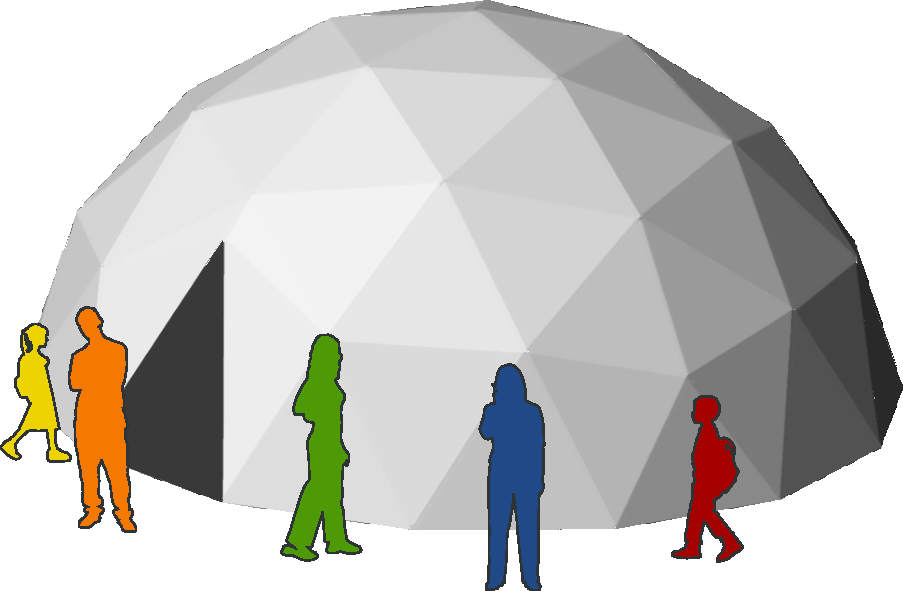
\includegraphics[width=7cm]{general.pdf}\\
	\vfill
}

%%%%%%%%%%%%%%%%%%%%%%%%%%%%%%%%%%%%%%%%%%%%%%%%%%%%%%%%%%%%%%%%%%%%%%%%%%%%%%%%%
%%%%%%%%%%%%%%%%%%%%%%%%%%%%%%%%%%%%%%%%%%%%%%%%%%%%%%%%%%%%%%%%%%%%%%%%%%%%%%%%%
\begin{document}

\maketitle
\clearpage
\tableofcontents

%%%%%%%%%%%%%%%%%%%%%%%%%%%%%%%%%%%%%%%%%%%%%%%%%%%%%%%%%%%%%%%%%%%%%%%%%%%%%%%%%
%%%%%%%%%%%%%%%%%%%%%%%%%%%%%%%%%%%%%%%%%%%%%%%%%%%%%%%%%%%%%%%%%%%%%%%%%%%%%%%%%

\section{Objet de la convention}

La présente convention précise le mode de gestion du dôme géodésique mutalisé
(ci-après désigné "le dôme") entre les associations Tetalab, Planète Sciences
Midi-Pyrénées et InCOGnu.

Le dôme est une structure métallique couverte d'une toile imperméable et
opaque, destinée en premier lieu à la projection vidéo hémisphérique.

Le dôme comprend :

\begin{itemize}

	\item Une structure métallique composée de 120 tubes d'aciers
de 25mm de diamètre ainsi que 46 boulons,

	\item Une toile hémisphérique pouvant couvrir le dôme,

	\item Un système de projection hémisphérique composé d'un video-projecteur
	haute-définition et d'une optique "fish-eye".

	\item 4 malles de rangement

\end{itemize}


Le dôme a une capacité stricte de 25 personnes, y compris l'encadrement.

\section{Signataires de la convention}

La présente convention est signée entre les trois associations Tétalab, Planète
Sciences Midi-Pyrénées et InCOGnu, représentées par leurs président(e)s
respectif(ve)s \presidenttetalab, \presidentplasci~et \presidentincognu.

Le Tetalab est...

InCOGnu est l'association des étudiants en sciences cognitives de la région
toulousaine. Ses principales activités incluent des rencontres entre étudiants,
entre chercheurs et grand-public, ainsi que des ateliers à destination du grand
public lors d'évènement comme La Semaine du Cerveau ou l'ExpoSciences.

Planète Sciences Midi-Pyrénées est l'antenne régional du réseau Planète
Sciences. C'est une association dont la vocation est la diffusion de la culture
scientifique auprès des jeunes. Ses principales thématiques sont les activités
spatiales, les sciences environementales, l'astronomie, la robotique.

\section{Réservation et utilisation du dôme}

Les trois associations disposent équitablement du dôme sur l'année.

Afin de permettre une utilisation partagée, un calendrier en ligne est mis en
place, sur lequel chacune des association peut réserver des plages de temps
d'utilisation. Une plage ne peut dépasser 2 semaines sans accord préalable des
trois associations.

Chaque association identifie et nomme un (ou de préférence deux) "responsable
dôme". Celui-ci est formé à l'installation du dôme, à son utilisation, et aux
consignes de sécurité.

À chaque utilisation, l'association utilisatrice est responsable du montage,
démontage et rangement du dôme. En cas de dégradation du matériel,
l'association utilisatrice doit prévenir les deux autres structures. Elle prend
à sa charge les éventuelles réparations, sauf accord avec les autres
associations.

Le lieu de stockage permanent du dôme est à Mix'Art Myrys, du fait de l'espace
disponible. A REDISCUTER...

À la fin de chaque année scolaire, une réunion entre les trois associations est
organisée pour faire le bilan de l'utilisation du dôme, et en revoir si
nécessaire les règles. D'autres réunions peuvent être organisées durant
l'année, à la demande d'une des associations.

\section{Modifications apportées au dôme}

En cas de modification substantielle apportée au dôme (modification de la
structure métallique, modification de la toile de couverture, adjonction d'un
module, etc.), un accord écrit de chacune des associations est nécessaire.

Les frais entrainés par cette modification sont à la charge de la structure
souhaitant effectuer la  modification, sauf accord entre les structures. De
plus, cette même structure à l'obligation de s'assurer de la conformité au 

\section{Sécurité}

Le dôme est une structure pouvant accueillir du public (ERP) de type CTS
(Chapiteaux, Tentes, Structures toiles). Sa capacité de 25 personnes le classe
en 5eme catégorie (moins de 50 personnes).

Un règlement de sécurité spécifique décrit les consignes de sécurité pour
l'utilisation du dôme avec le public.

En aucun cas le dôme peut être ouvert au public en l'absence d'un encadrant
issue d'une des trois associations, dûment formé à l'utilisation du dôme.

\section{Assurance}


\section{Intégration d'une structure tièrce dans la présente convention}

Après accord écrit des trois structures fondatrices, une nouvelle structure
peut être intégrée à la présente convention.

Le temps d'utilisation reste équitablement partagé entre toutes les structures.

\section{Retrait d'un des signataires}

Une structure peut se retirer de la présente convention à sa propre initiative.

Dans ce cas, elle ne peut prétendre à aucune des parties du dôme listées au
premier paragraphe de cette convention. Le dôme devient la pleine propriété des
structures restantes.

Convention signée le .............


\begin{center}
\begin{tabular}{ccc}
\presidenttetalab & \presidentincognu & \presidentplasci    
\end{tabular}
\end{center}

\end{document}

